\documentclass{beamer}
\usetheme{default} % You can change the theme as per your requirement
\usepackage{tikz}
\usepackage{amsmath}
\usepackage{pgfplots}
\usepackage{amsmath}
\usetikzlibrary{arrows.meta, positioning}


% \newtheorem{example}{}

% Additional packages (if required)
% \usepackage{...}

\title{Text Generation with MCMC}
\author{Shlok Mishra}
\date{\today} % or specific date

\begin{document}




\begin{frame}
    \titlepage
\end{frame}

\begin{frame}{Introduction to Language Models}
    \begin{itemize}
        \item \textbf{What are Language Models (LMs)?} \\
              Predict the likelihood of a sequence of words, enabling machines to generate and understand human languages.
        \item \textbf{Applications:}
              \begin{itemize}
                  \item Text generation
                  \item Sentiment analysis
                  \item Conversation AI
                  \item And more...
              \end{itemize}
        \item \textbf{Why are they important?} \\
              Key to advancing AI's ability to interact in human-like ways, driving innovations in automation, content creation, and beyond.
    \end{itemize}
\end{frame}

\begin{frame}{Examples of Advanced Language Models}
    \begin{columns}
        \column{0.33\textwidth}
        \centering
        
\includegraphics[width=0.8\linewidth]{chat-gpt.jpg}\\
        ChatGPT by OpenAI

        \column{0.33\textwidth}
        \centering
        
\includegraphics[width=0.8\linewidth]{gemini.png}\\
        Gemini by Google

        \column{0.33\textwidth}
        \centering
        
\includegraphics[width=0.8\linewidth]{llama.png}\\
        LLaMA by Meta
    \end{columns}
    \vfill
    \begin{itemize}
        \item ChatGPT, Gemini, and LLaMA represent the cutting-edge in language model technology, each contributing uniquely to the field.
        \item Their development by leading tech companies underscores the significant investment and interest in AI and NLP research.
    \end{itemize}
\end{frame}

\begin{frame}{Introduction to Neural Text Generation}
    \begin{block}{What is Neural Text Generation?}
        Neural Text Generation is the process of using neural networks to model the distribution of text sequences. This technology allows for the automatic creation of text that mimics human language patterns.
    \end{block}
    \begin{block}{Importance}
        It's a foundational technology for a range of applications, from chatbots and automated story generation to translation services and beyond.
    \end{block}
\end{frame}

\begin{frame}{The Mathematics Behind Text Generation}
    \begin{block}{Modeling Sequence Probability}
        The probability of a text sequence is decomposed into per-token conditional probabilities, parameterized by neural networks like transformers:
    \end{block}
    \begin{equation}
        p_{\theta} = \prod_{t=1}^{T} p_{\theta} (y_t | y_{<t}),
    \end{equation}
    where:
    \begin{itemize}
        \item $y = (y_1, \ldots, y_T)$ is a sequence of tokens, where a token is the smallest unit of text that holds meaning in the dataset. Depending on the preprocessing, a token can be a word, part of a word, a character, or a punctuation mark.
        \item $y_{<t}$ represents all tokens before the $t^{th}$ token, providing a context for predicting the next token.
        \item $\theta$ denotes the model parameters, which are learned from data to map sequences of tokens to probabilities.
    \end{itemize}
\end{frame}

\begin{frame}{Introduction to Constrained Text Generation}
    \begin{block}{Defining Constrained Text Generation}
        Constrained Text Generation focuses on producing text sequences that satisfy specific predefined constraints. These constraints can be categorized into:
    \end{block}
    \begin{itemize}
        \item \textbf{Hard constraints:} Must-include tokens or phrases.
        \item \textbf{Soft constraints:} Desired semantic similarities or thematic consistencies.
    \end{itemize}
\end{frame}

\begin{frame}{Conditioning on Constraints and Prompts}
    \begin{block}{Incorporating Constraints}
        Constraints are integrated directly into the generation model, allowing for text production that aligns with the set conditions, including conditioning on a specific prompt $x$.
    \end{block}
    \begin{equation}
        p_{\theta} (y|C, x) = \prod_{t=1}^{T} p_{\theta} (y_t | y_{<t}, C, x),
    \end{equation}
    where $C$ denotes the constraints, and $x$ is the given prompt guiding the generation process.
    \begin{block}{Goal}
        The ultimate goal is to generate text that is not only contextually and semantically coherent but also adheres closely to the predefined constraints and prompt $x$.
    \end{block}
\end{frame}

\begin{frame}{Lexically Constrained Text Generation}

    \begin{block}{Key Elements}
        \begin{itemize}
            \item \textbf{Fluency:} Ensures the text flows logically and naturally.
            \item \textbf{Keywords:} Predetermined words that must appear in the generated text.
        \end{itemize}
    \end{block}

    % Include the image with the example
    \begin{figure}
        \centering
        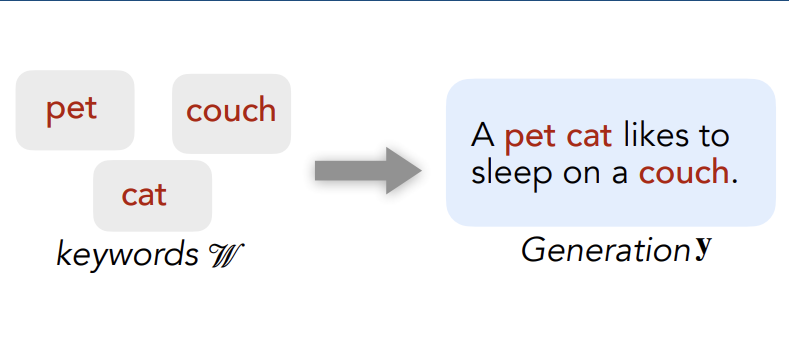
\includegraphics[width=0.8\textwidth]{constraint1.png}
        \caption{Example of lexically constrained text generation.}
    \end{figure}
\end{frame}

\begin{frame}{Abductive Reasoning in Text Generation}

    \begin{block}{Key Constraints}
        \begin{itemize}
            \item \textbf{Fluency:} The generated text must read smoothly and naturally, adhering to grammatical norms.
            \item \textbf{Past Coherence:} The text must logically follow from the provided past context, creating a seamless narrative transition.
            \item \textbf{Future Coherence:} The text should lead logically into the given future scenario, ensuring a coherent and believable progression of events.
        \end{itemize}
    \end{block}

    % Include the image with the example
    \begin{figure}
        \centering
        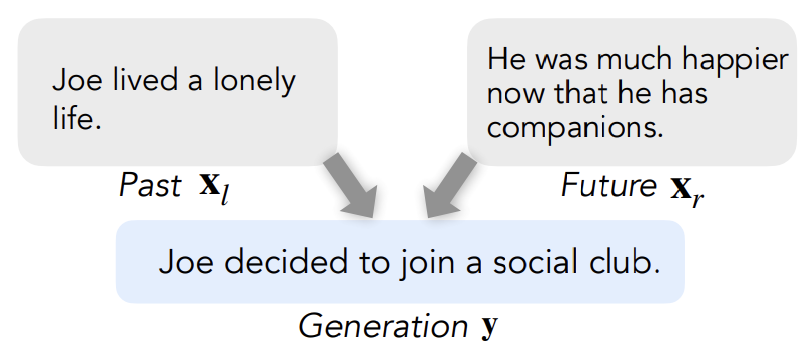
\includegraphics[width=0.8\textwidth]{constraint2.png}
        \caption{Example of abductive reasoning in text generation.}
    \end{figure}
\end{frame}

\begin{frame}{Counterfactual Reasoning in Text Generation}

    \begin{block}{Core Constraints}
        \begin{itemize}
            \item \textbf{Fluency:} Generated text must be smooth and grammatically correct.
            \item \textbf{Coherence:} The alternate narrative should logically follow from the original context, maintaining a coherent story or argument.
            \item \textbf{Minimal Edit:} Changes to the original text should be minimal, altering the narrative without extensive rewrites.
        \end{itemize}
    \end{block}

    % Include the image with the example
    \begin{figure}
        \centering
        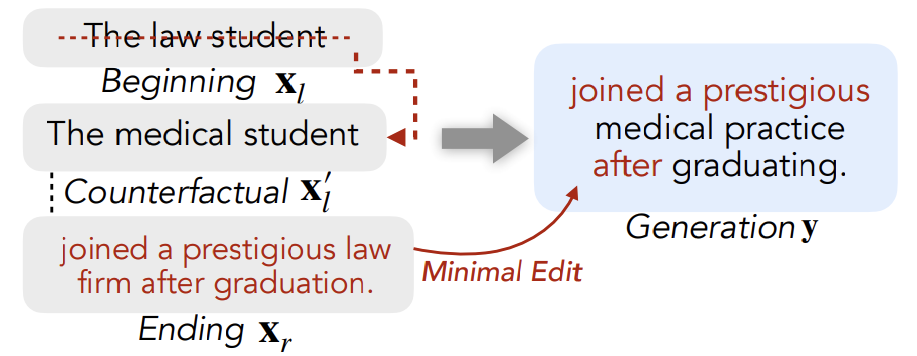
\includegraphics[width=0.8\textwidth]{constraint3.png}
        % \caption{Example of counterfactual reasoning in text generation.}
    \end{figure}
\end{frame}

\begin{frame}{Introduction to Energy-Based Models (EBMs)}
    \begin{block}{What is an Energy Function?}
        In the realm of text generation, an \textbf{energy function} $E(y)$ assesses the compatibility of a text sequence $y$ with specific constraints. Lower energy values signify a higher degree of adherence to these constraints, guiding the generation towards more desirable outcomes.
    \end{block}

    \begin{block}{Defining EBMs}
        EBMs offer a robust framework for utilizing energy functions to shape the distribution of generated text sequences. This approach is encapsulated in the Boltzmann distribution:
        \begin{equation}
            p(y) = \frac{\exp(-E(y))}{Z},
        \end{equation}
        where $E(y) \in \mathbb{R}$ represents the sequence's energy, and $Z$, the normalizing factor, ensures probabilities sum to 1.
    \end{block}
\end{frame}

\begin{frame}{Leveraging Energy Functions in EBMs}
    \begin{itemize}
        \item Energy functions $E(y)$ central to embedding multiple constraints in models.
              \begin{itemize}
                  \item Encodes fluency, coherence, and keyword inclusion directly into $E(y)$.
                  \item Sequences fulfilling constraints have lower energy.
              \end{itemize}
        \item EBMs' versatility key to their effectiveness.
              \begin{itemize}
                  \item Provide a unified system for incorporating diverse constraints.
                  \item Facilitate generation of contextually aligned and condition-compliant text.
                  \item Enhance text quality and broad applicability.
              \end{itemize}
    \end{itemize}
\end{frame}

\begin{frame}{Energy Function: Fluent Generation}
    \begin{center}
        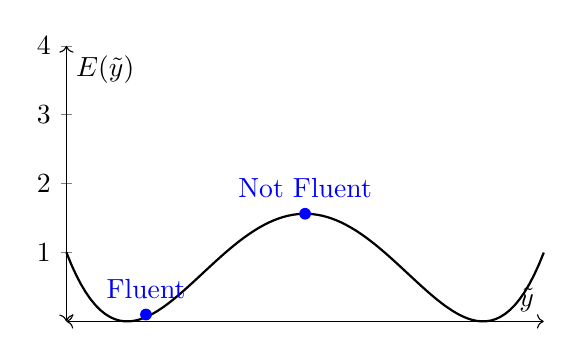
\begin{tikzpicture}
            \begin{axis}[
                    xlabel={$\tilde{y}$},
                    ylabel={$E(\tilde{y})$},
                    xmin=0, xmax=3,
                    ymin=0, ymax=4,
                    axis lines=middle,
                    axis line style=<->,
                    width=0.5\linewidth,
                    height=3.5cm,
                    scale only axis,
                    clip=false,
                    no marks,
                    xtick=\empty,
                    samples=100,
                ]
                \addplot+[black, thick, domain=0:3] {x^4 - 6*x^3 + 11*x^2 - 6*x + 1};
                \node[label={above:\textcolor{blue}{Not Fluent}},circle,fill,inner sep=1.5pt,blue] at (axis cs:1.5,{1.5^4 - 6*1.5^3 + 11*1.5^2 - 6*1.5 + 1}) {};
                \node[label={above:\textcolor{blue}{Fluent}},circle,fill,inner sep=1.5pt,blue] at (axis cs:0.5,0.1) {};
            \end{axis}
        \end{tikzpicture}
    \end{center}

    \begin{center}
        $f_{\overrightarrow{\text{LM}}}(\mathbf{\tilde{y}}) = \sum_{t=1}^{T} \sum_{v \in V} p_{\overrightarrow{\text{LM}}}(v|\mathbf{\tilde{y}}_{<t}) \log \text{softmax} (\mathbf{\tilde{y}}_t(v))$
    \end{center}

    \begin{itemize}
        \item \textbf{Not Fluent Example:} ``I has a dog where is curious.''
        \item \textbf{Fluent Example:} ``I have a dog that is very curious.''
    \end{itemize}

\end{frame}

\begin{frame}{Energy Function: Keyword Emphasis}
    \begin{center}
        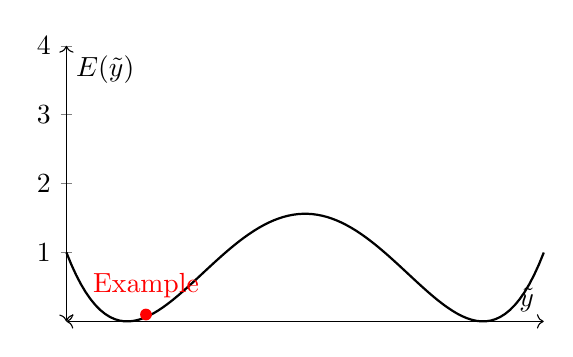
\begin{tikzpicture}
            \begin{axis}[
                    xlabel={$\tilde{y}$},
                    ylabel={$E(\tilde{y})$},
                    xmin=0, xmax=3,
                    ymin=0, ymax=4,
                    axis lines=middle,
                    axis line style=<->,
                    width=0.5\linewidth,
                    height=3.5cm,
                    scale only axis,
                    clip=false,
                    no marks,
                    xtick=\empty,
                    samples=100,
                ]
                \addplot+[black, thick, domain=0:3] {x^4 - 6*x^3 + 11*x^2 - 6*x + 1};
                \node[label={above:\textcolor{red}{Example}},circle,fill,inner sep=1.5pt,red] at (axis cs:0.5,0.1) {};
            \end{axis}
        \end{tikzpicture}
    \end{center}

    \begin{equation}
        f_{\text{sim}}(\tilde{\mathbf{y}}; \mathbf{y}^*) = \text{ngram-match}(\tilde{\mathbf{y}}, \mathbf{y}^*),
    \end{equation}

    \begin{itemize}
        \item \textbf{Example with Keywords:} ``My dog liked to \textcolor{red}{sleep} on a \textcolor{red}{couch}.''
        \item \textbf{Keywords} (\(\mathbf{y}^*\)): \{\textcolor{red}{sleep}, \textcolor{red}{couch}\}
    \end{itemize}

\end{frame}

\begin{frame}{Coherence Constraints: Foundation}
    \begin{block}{Coherence Constraint Equation}
        \begin{equation}
            f_{pred}(\mathbf{\tilde{y}}; \mathbf{x_r}) = \sum_{k=1}^{K} \log {p}_{\overrightarrow{LM}}({x_{r,k}}|\mathbf{\tilde{y}}, {\mathbf{x}_{r,<k}}),
        \end{equation}
    \end{block}
    \begin{block}{Example Setup for Coherence}
        Illustrating the function of coherence constraints using a fraction-like representation:
        \begin{itemize}
            \item Text Generation Objective (?): Generate text $\mathbf{\tilde{y}}$ that logically precedes or follows the context.
            \item Contextual Right Side ($\mathbf{x_r}$): "I love my cat."
        \end{itemize}
        This setup aims to generate a coherent sequence that aligns with the given context, $\mathbf{x_r}$.
    \end{block}
\end{frame}


\begin{frame}{Coherence Constraints: Visualization}
    \begin{center}
        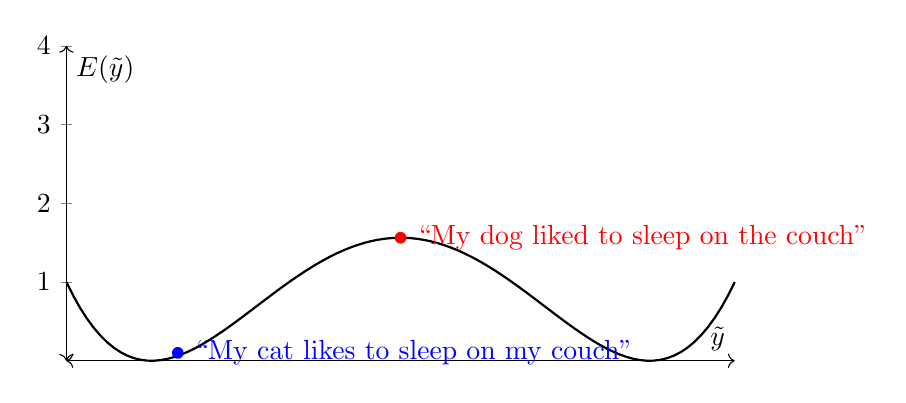
\begin{tikzpicture}
            \begin{axis}[
                    xlabel={$\tilde{y}$},
                    ylabel={$E(\tilde{y})$},
                    xmin=0, xmax=3,
                    ymin=0, ymax=4,
                    axis lines=middle,
                    axis line style=<->,
                    width=0.7\linewidth,
                    height=4cm,
                    scale only axis,
                    clip=false,
                    no marks,
                    xtick=\empty,
                    samples=100,
                ]
                \addplot+[black, thick, domain=0:3] {x^4 - 6*x^3 + 11*x^2 - 6*x + 1};
                \node[label={right:\textcolor{blue}{``My cat likes to sleep on my couch''}},circle,fill,inner sep=1.5pt,blue] at (axis cs:0.5,0.1) {};
                \node[label={right:\textcolor{red}{``My dog liked to sleep on the couch''}},circle,fill,inner sep=1.5pt,red] at (axis cs:1.5,{1.5^4 - 6*1.5^3 + 11*1.5^2 - 6*1.5 + 1}) {};
            \end{axis}
        \end{tikzpicture}
    \end{center}

    \textbf{Interpreting the Points:}
    \begin{itemize}
        \item The \textcolor{blue}{blue point} represents a sentence coherent with the right context "I love my cat," hence lower energy.
        \item The \textcolor{red}{red point} represents a less coherent sentence, not perfectly aligning with the context, thus higher energy.
    \end{itemize}
\end{frame}


\begin{frame}{Total Energy and Induced Distribution in Text Generation}
    \begin{block}{Energy Function and Induced Distribution}
        \begin{itemize}
            \item The set of constraints induces a distribution over text, formulated in an energy-based form as:
                  \begin{equation*}
                      p(y) = \frac{\exp\left( \sum_{i} \lambda_{i}f_{i}(y) \right)}{Z},
                  \end{equation*}
                  where $\lambda_{i} \geq 0$ is the weight of the $i^{th}$ constraint, and $Z$ is the normalizing factor.

            \item Here, the energy function $E(y)$ is defined as:
                  \begin{equation*}
                      E(y) := -\sum_{i} \lambda_{i}f_{i}(y),
                  \end{equation*}
                  which aggregates the weighted sum of various energy components, each reflecting a specific constraint.
        \end{itemize}
    \end{block}

    % \begin{block}{Specific Constraints and Energy-Based Model (EBM)}
    %     These constraints translate into meaningful components such as:
    %     \begin{itemize}
    %         \item \textcolor{blue}{Fluent Generation}
    %         \item \textcolor{red}{Keyword Constraints}
    %         \item \textcolor{green}{Future Context Constraints}
    %         \item \ldots
    %     \end{itemize}
    %     Consequently, the energy function $E(y)$ is converted into a probability distribution for an Energy-Based Model (EBM), enabling the generation of text that complies with predefined conditions.
    % \end{block}
\end{frame}

\begin{frame}{Challenges in Constrained Generation: Energy Functions}
    \begin{block}{Complex High-Dimensional Energy Functions}
        The energy function $E(y)$ in constrained text generation presents significant challenges:
        \begin{itemize}
            \item The \textbf{normalizing factor $Z$} is intractable due to summation over all possible states, complicating direct sampling efforts.
            \item Text sequences $y$ are \textbf{inherently discrete}, making traditional Markov Chain Monte Carlo (MCMC) methods like Gibbs sampling less effective due to slow convergence in high-dimensional spaces.
        \end{itemize}
    \end{block}
\end{frame}

\begin{frame}{Solutions: Continuous Approximation and Langevin Dynamics}
    \begin{block}{Addressing Sampling Challenges}
        To navigate the complexity of sampling from high-dimensional energy functions:
        \begin{itemize}
            \item \textbf{Continuous Approximation:} Transforming the discrete sequence $y$ into a continuous space allows for the application of more sophisticated sampling techniques.
            \item \textbf{Langevin Dynamics:} A gradient-based MCMC method that exploits the continuous approximation to perform efficient sampling by utilizing the gradient information of $E(y)$.
        \end{itemize}
    \end{block}

    \begin{block}{Advantages}
        These strategies enable effective and efficient exploration of the energy landscape, facilitating the generation of text that adheres to the specified constraints while overcoming the limitations of discrete sequence spaces.
    \end{block}
\end{frame}


\begin{frame}{Gradient-Based MCMC for Efficient Sampling}
    \begin{block}{Langevin Dynamics}
        The Langevin dynamics update rule for sampling is given by:
        \begin{equation}
            \tilde{\boldsymbol{y}}^{(n+1)} \leftarrow \tilde{\boldsymbol{y}}^{(n)} - \eta \nabla_{\tilde{\boldsymbol{y}}} E(\tilde{\boldsymbol{y}}^{(n)}) + \epsilon^{(n)},
        \end{equation}
        where $\epsilon^{(n)} \sim \mathcal{N}(0, \sigma)$ is the noise term at iteration $n$, and $\eta$ is the step size.
    \end{block}

    \begin{block}{Efficient Sampling}
        Gradient-based MCMC methods like Langevin dynamics allow for more efficient sampling from complex distributions by utilizing the gradient of the energy function $\nabla_{\tilde{\boldsymbol{y}}} E(\tilde{\boldsymbol{y}})$. This approach leverages gradient information to navigate the energy landscape and generate samples that adhere to the desired constraints.
    \end{block}
\end{frame}


\begin{frame}{From Discrete Tokens to Continuous Soft Sequences}
    \begin{block}{Soft Sequence Representation}
        Rather than operating on discrete tokens, we construct an energy function over a soft sequence of continuous vectors:
        \[
            \tilde{\boldsymbol{y}} = (\tilde{\boldsymbol{y}}_1, \ldots, \tilde{\boldsymbol{y}}_T),
        \]
        where each $\tilde{\boldsymbol{y}}_t \in \mathbb{R}^V$ represents a position in the sequence with $V$ being the vocabulary size.
    \end{block}

\end{frame}

\begin{frame}{Example: Soft Sequence in Natural Language Processing}
    \begin{block}{Model's Logits at Time Step $t$}
        Given a small vocabulary, the neural network model produces logits for each word at time step $t$:
    \end{block}

    \begin{table}
        \centering
        \begin{tabular}{lcc}
            \textbf{Word} & \textbf{Logit} & \textbf{Probability} \\
            \hline
            ``the''       & 2              & 0.12                 \\
            ``cat''       & 5              & 0.79                 \\
            ``sat''       & 1              & 0.07                 \\
            ``mat''       & -1             & 0.02                 \\
        \end{tabular}
        \caption{Logits and probability distribution for each word in the vocabulary.}
    \end{table}

    \begin{block}{Soft Sequence at Time Step $t$}
        The continuous representation of the model's prediction at time $t$ is a vector indicating the probability of each word:
        \[
            [0.12, 0.79, 0.07, 0.02]
        \]
        With this representation, ``cat'' is the most probable next word with a probability of 0.79.
    \end{block}
\end{frame}

\begin{frame}{Discretization of Soft Sequence After MCMC}
    \begin{block}{Utilizing the Language Model as a Guardian}
        \begin{itemize}
            \item Post-MCMC, we discretize the continuous soft sequence \(\tilde{y}\) into discrete tokens \(y\).
            \item The language model (e.g., GPT2-XL) guides the selection of discrete tokens from the soft sequence.
        \end{itemize}
    \end{block}

    \begin{block}{Top-k Filtering Method}
        At each position \(t\), the language model suggests the top-k most likely candidate tokens given the preceding tokens:
        \begin{itemize}
            \item Denote the top-k candidate set as \(\nu_k^t\).
            \item The discrete token \(y_t\) is chosen as the one with the highest logit from \(\tilde{y}_t\) within the top-k set:
                  \begin{equation}
                      y_t = \text{arg max}_{v \in \nu_k^t} \tilde{y}_t(v).
                  \end{equation}
        \end{itemize}
    \end{block}

\end{frame}

\begin{frame}{Challenges in Implementation of COLD Decoding}
    \begin{itemize}
        \item Publicly available implementation: 
\includegraphics[scale=0.2]{github-mark.png} \footnote{\url{https://github.com/qkaren/COLD_decoding}}

        \item Extensive codebase: Tens of Thousands of lines to navigate across multiple files.
        \item Resource-intensive: Requires high-memory GPUs beyond personal computing capabilities.
        \item Acknowledgment: Gratitude to Prof. Dootika Vats for providing necessary resources.
        \item Learning curve: Complex use of PyTorch and advanced NLP concepts.
        \item Time constraint: Difficulty in mastering sophisticated codebase rapidly.
    \end{itemize}
\end{frame}

\begin{frame}{Langevin MCMC in High-Dimensional Text Generation}

    \begin{block}{Langevin MCMC Fundamentals}
        \begin{itemize}
            \item Inspired by particle dynamics in physics.
            \item Balances deterministic drift with stochastic exploration.
        \end{itemize}
    \end{block}

    \begin{block}{Update Formula}
        The Langevin MCMC update rule is given by:
        \begin{equation}
            x_{t+1} = x_t + \frac{\epsilon^2}{2} \nabla \log p(x_t) + \epsilon Z_t,
        \end{equation}
    \end{block}

    \begin{block}{Efficiency and Applications}
        \begin{itemize}
            \item Effective in high-dimensional sampling.
            \item Widely applicable in machine learning and physics.
            \item Utilizes gradient information for enhanced convergence.
        \end{itemize}
    \end{block}
\end{frame}

\begin{frame}{Issue with Langevin Dynamics in COLD Decoding}
    \begin{block}{Discrepancy in Implementation}
        \begin{itemize}
            \item The COLD decoding paper claims to use Langevin dynamics for text generation.
            \item However, the actual implementation utilizes the Adam optimizer.
            \item Adam optimizer inherently adjusts learning rates adaptively.
            \item This contradicts the requirements of Langevin MCMC where a fixed ratio between the learning rate and noise is crucial.

        \end{itemize}
    \end{block}

    \begin{block}{Paper's Claim vs. Reality}
        The title suggests a methodology based on Langevin dynamics, but the use of Adam calls into question the fidelity of the Langevin process in their approach.
    \end{block}
\end{frame}

\begin{frame}{Barker Proposal MCMC for Enhanced Sampling}
    \begin{block}{Acceptance Probability}
        For perturbation \(z\) from \(z \sim \mathcal{N}(0, \sigma^2)\), the acceptance probability \(\alpha\) is:
        \begin{equation}
            \alpha = \frac{1}{1+e^{-z \cdot \nabla_{y} E(y_k)}},
        \end{equation}
        balancing exploration and exploitation based on the energy gradient.
    \end{block}

    \begin{block}{Update Rule}
        The state update is probabilistically determined:
        \begin{equation}
            y_{k+1} =
            \begin{cases}
                y_k + z & \text{with probability } \alpha,   \\
                y_k - z & \text{with probability } 1-\alpha.
            \end{cases}
        \end{equation}
        This rule adapts to both the energy landscape and stochastic perturbations.
    \end{block}
\end{frame}

\begin{frame}{Results - Performance of SGD and Barker MCMC}
    \begin{block}{Observations}
        \begin{itemize}
            \item Direct implementations of SGD and Barker Proposal MCMC demonstrated poor performance in our tests.
            \item Contrastingly, Adam optimizer showed more stable loss trajectories.
        \end{itemize}
    \end{block}

    \begin{block}{Figure: Loss Trajectories Comparison}
        \begin{figure}
            \centering
            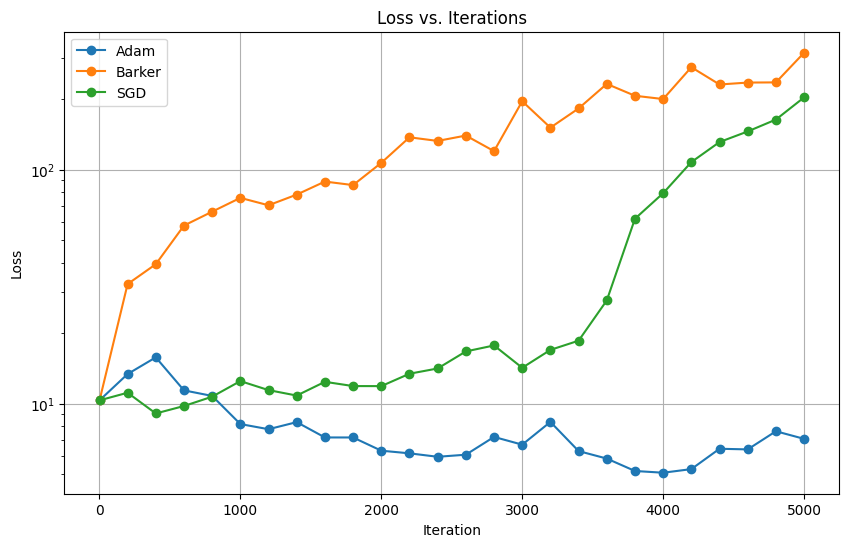
\includegraphics[width=0.75\textwidth]{seed12.png}
            \caption{Loss trajectories for Adam, SGD, and Barker with seed 12.}
        \end{figure}
    \end{block}
\end{frame}

\begin{frame}{Future Directions in Sampling Methodologies}
    \begin{itemize}
        \item Thorough investigation into why Adam optimizer outperforms in certain contexts.
        \item Identify specific challenges with Langevin and Barker sampling techniques.
        \item Collaborative research with Professor Vats to deepen our understanding of these issues.
        \item Strategy: Construct and test models from scratch on a manageable scale.
        \item Focus on experimenting with different sampling techniques to identify effective strategies.
        \item Engage deeply with NLP aspects of the research to uncover foundational insights.
        \item Goal: Achieve a nuanced understanding of text generation challenges using MCMC methods.
    \end{itemize}
\end{frame}


\begin{frame}{Thank You}
    \centering
    \LARGE Thank You for Your Attention!\\[10pt]
    \normalsize Questions?
\end{frame}

% \bibliographystyle{plain}  % Choose an appropriate style
% \bibliography{references}  % Replace "your-bib-file" with the actual name of your .bib file (without the .bib extension)


\end{document}
